\section{Análisis}

\subsection{Contexto}
\subsubsection{Descripción General}
Como todo proyecto el paso inicial es un análisis del objetivo a realizar, y este caso no es la excepción. La información utilizada para este análisis consiste en una explicación concisa de los requerimientos necesarios de la aplicación, principalmente mecánicas y características que debe contener la versión final.\\
El resultado del análisis llevó a una descripción propia del proyecto, el resultado final es una aplicación que funcione como herramienta interactiva basada en una enseñanza de exploración y el contenido que esta acción entrega. La parte lúdica del aprendizaje se ve con la implementación de un sistema inspirado en juegos de mesa donde un numero plural de usuarios toman turnos para realizar acciones y avanzar en un mapa para llegar a una meta final. Cada turno se les entrega a los jugadores una imagen en 360 grados de un área o paisaje en particular y una cantidad de conceptos escogidos al azar (estas palabras son encontradas en una base de datos) con esto los usuarios tendrán que concebir una historia usando los datos mencionados. Al final todos tendrán que votar por otro usuario que consideren haber creado la mejor historia, el usuario ganador avanza un espacio y se sigue la misma idea cada turno hasta que uno llegue al final.\\
En cuanto a los problemas mencionados en el punto 1.1.2 se tomó la esquematización de estos y se analizaron con profundidad. La base de datos a utilizar debe centrarse en una cantidad reducida de usuarios (cuantos jugadores simultáneos se encuentran), también se llegó a la conclusión de que cada usuario cuenta con su propio dispositivo (un smartphone) por lo que se requerirá uso de internet para facilitar los datos a los usuarios. El análisis del proyecto y de la situación del equipo de desarrollo encuentra que el uso de Android studio (con el lenguaje de kotlin) y la implementación de firebase a este es la opción mas viable.\\
El diseño de la aplicación lleva a la conclusión de comenzar la estructura principal de este (encontrado en el caso de estudio entregado al equipo) dándole una mayór importancia la implementación las mecánicas claves recibidas, asegurándose de que estas funcionen sin problemas antes de ampliar o expandir el desarrollo del proyecto.\\
Lo que respecta a material audiovisual el equipo encarga en las ultimas fases de desarrollo un tiempo en particular para la búsqueda e implementación de sonidos o imágenes necesarias, y al igual que los otros casos, dándole mayor importancia a las direcciones entregadas al equipo, en este caso siendo el uso de imágenes en 360 grados en la aplicación.

\subsubsection{Descripción de Clientes y Usuarios:}
Luego de un análisis realizado en base a la información entregada del resultado esperado por la aplicación se a encontrado un perfil definido para tanto clientes como usuarios.\\
Los clientes son parte del laboratorio mauletec y fueron concretados como un grupo centrado en el turismo, una de las principales mecánicas presentadas. En específico, la vista de paisajes y lugares geográficos en 360 grados le interesa a un grupo enfocado en turismo; como forma de enseñar los paisajes de una zona o región en particular. El otro enfoque encontrado en la aplicación que puede llamar la atención para un cliente es la mecánica de crear historias en base a palabras encontradas en una base de datos, tomando con mayor atención la parte literaria de juego centrada en la creatividad del usuario, pero siendo usada como forma de enseñanza. Para resumir, la motivacion principal de nuestro cliente con este proyecto es dar a cnocer la cultura de la region del maule de manera lúdica y entretenida al publico general.\\
Por otro lado, durante el desarrollo del software los usuarios tomaron un enfoque más genérico que el de los clientes, se encontró que en cualquier caso estos tenían requerimientos  simples ya que lo más importante para ellos es que la aplicación sea de uso sencillo. El usuario objetivo se identificó como un individuo o individua con un conocimiento básico de tecnología, tomando en cuenta de que la plataforma utilizada es de smartphones. Ademas de contar con un dispositivo que posea un sistema operativo que permita instalar y usar la aplicación, se requiere que el usuario entienda el concepto de identificarse de forma virtual con su correo electronico ademas de entender las reglas básicas del juego. Además, este debe tener un conocimiento literario de enseñanza básica como mínimo, tomando en cuenta de que la interacción principal de parte del usuario es crear y contar una historia en base a un grupo de palabras entregadas, En definitiva, nuestro usuario es cualquier persona natural can lal capacidades necesarias para utilizar la tecnologia basica y con capacidades de comprencion y habla al nivel de un niño en enseñanza basica.
\newpage
\subsection{Especificación de Requerimientos}
\subsubsection{Funciones del Sistema}

Tablas de funciones evidentes del sistema
\begin{table}[H]
    \begin{center}
        \begin{tabular}{| m{2.3cm} | m{5cm} | m{8cm} |}        
        	\hline 
        	Identificador & Nombre & Descripción\\
        	\hline
        	F.1.01 & Registrar nuevo usuario & Permitir al usuario ingresar con una cuanta nueva\\
        	\hline
        	F.1.02 & Realizar autentificacion con correo & Autorizar el ingreso del ususario por medio de reconocimiento con cuenta de correo\\
        	\hline
        	F.1.03 & Realizar autentificacion con contraseña & Autorizar el ingreso del ususario por medio de reconocimiento con contraseña\\
        	\hline
        	F.1.04 & Realizar autentificacion con Gmail & Autorizar el ingreso del ususario por medio de reconocimiento con cuenta de gmail\\
        	\hline
        	F.1.05 & Mostrar imagenes en 360° & Principal caracteristica del sistema que permite mostrar por pantalla una imagen es 360°\\
        	\hline
        	F.1.06 & Sistema de turnos & Mecánica principal del juego para que todos los usuarios participen\\
        	\hline
        	F.1.07 & Generar lista de palabras & Se genera una lista de palabras sacadas de la base de datos\\
        	\hline
        	F.1.08 & Mostrar lista de palabras & Le muestra al usuario la lista de palabras generadas para darle sentido al juego\\
        	\hline
        	F.1.09 & Multijugador global & Función del sistema que permite a varios usuarios jugar una misma partida\\
        	\hline
        \end{tabular}
    \caption{Funciones evidentes}
    \end{center}
\end{table}

Tablas de funciones ocultas del sistema
\begin{table}[H]
    \begin{center}
        \begin{tabular}{| m{2.3cm} | m{5cm} | m{8cm} |}        
        	\hline 
        	Identificador & Nombre & Descripción\\
        	\hline
        	F.2.01 & Cargar imagenes en 360° & Sube las imagenes para ser usadas luego por la aplicación\\
        	\hline
        	F.2.02 & Crear base de datos para palabras & Se crea y guarda una lista de palabras previamente analizadas para ser usadas en el juego\\
        	\hline
        	F.2.03 & Crear base de datos para puntajes & Se almacenan los puntajes en la base de datos para ser analizados luego\\
        	\hline
        \end{tabular}
    \caption{Funciones ocultas}
    \end{center}
\end{table}

Tablas de funciones supérfluas del sistema
\begin{table}[H]
    \begin{center}
        \begin{tabular}{| m{2.3cm} | m{5cm} | m{8cm} |}        
        	\hline 
        	Identificador & Nombre & Descripción\\
        	\hline
        	F.3.01 & Generar una tabla de puntajes & Se muestran al jugador los puntajes ordenados de manera ascendente\\
        	\hline
        \end{tabular}
    \caption{Funciones supérfluas}
    \end{center}
\end{table}
\newpage
\subsubsection{Atributos del Sistema}
Los atributos del sistema son las cualidades con las que cuenta un software, y responden a las caracteristicas con 5 factores de calidad  que son: Funcionalidad, usabilidad, confiabilidad, prestación y soporte; mas comunmente llamado como "modelo FURPS+" por sus iniciales en inglés.\\
Las cualidades ya mencionadas cubren los factores de calidad y los atributos, restricciones de diseño y requerimientos de implementación, físicos y de interfaz. El unico contratiempo de este modelo, es que no abarca la portabilidad de los productos software que se consideran, esto es una limitacion debido a que no se tienen en cuenta las exigencia del dispositivo.

Tabla de atributos del sistema
\begin{table}[H]
    \begin{center}
        \begin{tabular}{| m{2.3cm} | m{3.5cm} | m{10cm} |}        
        	\hline 
        	Identificador & Nombre & Descripción\\
        	\hline
        	A.01 & Intuitiva & De fácil entendimiento. El usuario final debe saber que hacer o como empezar a jugar sin mucha complejidad\\
        	\hline
        	A.02 & Optimizado & La aplicación debe usar recursos del celular solo de ser sumamente necesario\\
        	\hline
        	A.03 & Baja frecuencia de fallos & El Programa no debe presentar mas de cuatro fallos al mes\\
        	\hline
        	A.04 & Facilidad de configuración & El usuario debe poder tener la aplicación como a el más le acomode y anexada a su email personal de preferencia\\
        	\hline
        	A.05 & Facilidad de mantenimiento & A los programadores y gente encargada de mantener la aplicación funcionando se les debe hacer sencillo ingresar al codigo, entenderlo y aplicar las reparaciones\\
        	\hline
        \end{tabular}
    \caption{Atributos del sistema}
    \end{center}
\end{table}

\subsubsection{Atributos por Función}
\begin{table}[H]
    \begin{center}
        \begin{tabular}{| l | m{6cm} | m{6cm} |}        
        	\hline 
        	Ref\# & Función & Atributo asociado\\
        	\hline
        	R1.1 & F.1.01 & Facilidad de configuración\\
        	\hline
        	R1.2 & F.1.02, F.1.03, F.1.04 & Facilidad de configuración\\
        	\hline
        	R1.3 & F.1.05 & Intuitiva\\
        	\hline
        	R1.4 & F.1.06 & Intuitiva\\
        	\hline
        	R1.5 & F.1.07, F.1.08 & Intuitiva\\
        	\hline
        	R1.6 & F.1.09 & Facilidad de configuración\\
        	\hline
        	R1.7 & F.2.01 & Facilidad de configuración\\
        	\hline
        	R1.8 & F.2.02, F.2.03 & Facilidad de mantenimiento\\
        	\hline
        \end{tabular}
    \caption{Atributos por función}
    \end{center}
\end{table}
\newpage
\subsection{Actores}
\begin{enumerate}[1.]
	\item Jugador : El fin último de la aplicación en entretener al público, por lo que todos los jugadores, es decir, aquellos que frecuenten la aplicación, deben ser siempre nuestro punto de ancla a la hora de generar ideas para nuestro software.
	\item Google FireBase: Google FireBase es uno de los actores que permite la comunicación entre distintas herramientas, y así facilitar la funcionalidad del software. Algunas de las herramientas que utilizamos a través de FireBase son:
	\begin{enumerate}[a)]
		\item Base de Datos : La aplicación debe mantener contacto con la base de datos de forma directa, para poder acceder a las palabras, imágenes, usuarios, etc.
		\item Gmail : Herramienta principal para identificar al usuario por medio de correo electrónico.
	\end{enumerate} 
\end{enumerate}
\newpage
\subsection{Casos de Uso}
En las siguienetes subsecsiones identificaremos y analizaremos algunos de los casos de uso detectadosy como estos tienen relacion con los autore, requisitos, y funciones del sistema vistos con anterioridad en este informe.
\subsubsection{Caso de Uso Esencial}
\begin{table}[H]
    \begin{center}
        \begin{tabular}{| l | m{12cm} |}        
        	\hline 
        	Identificador & 1\\
        	\hline
        	Caso de Uso & Jugar un turno de Conquista Turística
360°\\
        	\hline
        	Actores & Jugador\\
        	\hline
        	Propósito & Jugar un turno\\
        	\hline
        	Tipo & Primario y escencial\\
        	\hline
        	Descripción & El jugador recibe por pantalla palabras que debe usar para crear una historia. El sistema recibe el feedback de los demas jugador y según lo que puntue este, avanza o no.\\
        	\hline
        	Referencias Cruzadas & R1.4 ,R1.5 ,R1.6\\
        	\hline
        \end{tabular}
    \caption{Primer caso de uso}
    \label{Caso_de_uso_1}
    \end{center}
\end{table}

\begin{longtable}[H]{| m{8cm} | m{8cm} |}
\hline 
\textbf{Acción de los actores} & \textbf{Respuesta del sistema}\\
\hline 
1.-Este caso de uso comienza cuando el ususario inicia un turno de juego & 2.-La GUI le presenta al ususario un listado de palabras\\
\hline
3.-El usuario crea una historia usando las palabras presentadas & \\
\hline
4.-Los otros participantes califícan la historia & 5.-El sistema recibe las puntuaciones y procesa la información\\
\hline
& 6.-El jugador recibe una calificacion positiva y avanza al siguiente punto\\
\hline
\multicolumn{2}{| l |}{\textbf{Flujo alternativo}} \\
\hline
\multicolumn{2}{| m{16cm} |}{Línea 6.-El jugador recibe una calificacion negativa y se mantien en su pocisión hasta la siguiente ronda}\\
\hline
\caption{Descripción de procesos caso de uso N°1}
\end{longtable}

\begin{table}[H]
    \begin{center}
        \begin{tabular}{| l | m{12cm} |}        
        	\hline 
        	Identificador & 2\\
        	\hline
        	Caso de Uso & Iniciar sesión\\
        	\hline
        	Actores & Jugador y FireBase\\
        	\hline
        	Propósito & Entrar en su cuenta personal\\
        	\hline
        	Tipo & Primario y Real\\
        	\hline
        	Descripción & El jugador abre la aplicación he ingresa sus datos, la aplicación los recibe y los compara en la base de datos a traves del FireBase, si la informacion es correcta el jugador ingresa a la pantalla principal \\
        	\hline
        	Referencias Cruzadas & R1.1 ,R1.2\\
        	\hline
        \end{tabular}
    \caption{Segundo caso de uso}
    \label{Caso_de_uso_2}
    \end{center}
\end{table}

\begin{longtable}[H]{| m{8cm} | m{8cm} |}
\hline 
\textbf{Acción de los actores} & \textbf{Respuesta del sistema}\\
\hline 
1.-Este caso de uso comienza cuando el usuario abre la aplicación & 2.-La GUI le presenta al ususario un formulario de usuario y contraseña para ser rellenado\\
\hline
3.-El usuario rellena los campos señalados & 4.-El sistema verifica la información a traves del firebase\\
\hline
& 5.-La aplicación recibe los datos del firebase y accede a la pantalla principal\\
\hline
\multicolumn{2}{| l |}{\textbf{Flujo alternativo}} \\
\hline
\multicolumn{2}{| m{16cm} |}{Línea 2.-Se identifica que el usuario ya habia ingresado con enterioridad y la aplicacion accede directamente a la pantalla principal}\\
\hline
\multicolumn{2}{| m{16cm} |}{Línea 5.-Se identifica que los datos ingresados son incorrectos y la aplicacion le envia feedback al usuario}\\
\hline
\caption{Descripción de procesos caso de uso N°2}
\end{longtable}

\begin{table}[H]
    \begin{center}
        \begin{tabular}{| l | m{12cm} |}        
        	\hline 
        	Identificador & 3\\
        	\hline
        	Caso de Uso & Generar lista de palabras\\
        	\hline
        	Actores & Jugador y FireBase\\
        	\hline
        	Propósito & Entregar palabras para que el jugador pueda intervenir\\
        	\hline
        	Tipo & Primario y escencial\\
        	\hline
        	Descripción & El jugador toca la imagen 360° y la aplicacion accede a la base de datos a traves del FireBase, busca 4 palabras aleatorias y se las muestra al jugador por pantalla\\
        	\hline
        	Referencias Cruzadas & R1.3 ,R1.5\\
        	\hline
        \end{tabular}
    \caption{Tercer caso de uso}
    \label{Caso_de_uso_3}
    \end{center}
\end{table}

\begin{longtable}[H]{| m{8cm} | m{8cm} |}
\hline 
\textbf{Acción de los actores} & \textbf{Respuesta del sistema}\\
\hline 
1.-Este caso de uso comienza cuando el ususario Interactua con la imagen 360° & 2.-El software accede a la base de datos a traves del firebase\\
\hline
& 3.-Se buscan y seleccionan palabras al azar\\
\hline
& 4.-Se le presenta esta lista al usuario\\
\hline
\caption{Descripción de procesos caso de uso N°3}
\end{longtable}

\begin{table}[H]
    \begin{center}
        \begin{tabular}{| l | m{12cm} |}        
        	\hline 
        	Identificador & 4\\
        	\hline
        	Caso de Uso & Mostrar imagen 360°\\
        	\hline
        	Actores & Jugador\\
        	\hline
        	Propósito & Retroalimentar al jugador \\
        	\hline
        	Tipo & Primario y escencial\\
        	\hline
        	Descripción & Cuando el jugador conquista una posición, avanza a la siguiente y el programa le presenta a traves de una imagen 360° su nuevo objetivo\\
        	\hline
        	Referencias Cruzadas & R1.3\\
        	\hline
        \end{tabular}
    \caption{Cuarto caso de uso}
    \label{Caso_de_uso_4}
    \end{center}
\end{table}

\begin{longtable}[H]{| m{8cm} | m{8cm} |}
\hline 
\textbf{Acción de los actores} & \textbf{Respuesta del sistema}\\
\hline 
1.-Este caso de uso comienza cuando el jugador conquista una pocision y avanza a la siguiente & 2.-La GUI le presenta al ususario la nueva imagen 360°\\
\hline 
\caption{Descripción de procesos caso de uso N°4}
\end{longtable}

\begin{table}[H]
    \begin{center}
        \begin{tabular}{| l | m{12cm} |}        
        	\hline 
        	Identificador & 5\\
        	\hline
        	Caso de Uso & Mostrar tabla de puntajes\\
        	\hline
        	Actores & Jugador y FireBase\\
        	\hline
        	Propósito & Retroalimentar al jugador\\
        	\hline
        	Tipo & Secundario y real\\
        	\hline
        	Descripción & El jugador accede a la tabla de puntajes y el programa a su ves ingresa a la base de datos a traves del FireBase donde estan almacenados todos los puntajes y se los presenta al jugador de manera ordenada\\
        	\hline
        	Referencias Cruzadas & R1.8\\
        	\hline
        \end{tabular}
    \caption{Quinto caso de uso}
    \label{Caso_de_uso_5}
    \end{center}
\end{table}

\begin{longtable}[H]{| m{8cm} | m{8cm} |}
\hline 
\textbf{Acción de los actores} & \textbf{Respuesta del sistema}\\
\hline 
1.-Este caso de uso comienza cuando el jugador accede a la tabla de puntajes & 2.-El sistema recibe la orden he ingresa a la base de datos\\
\hline
& 3.-El sistema adquiere los puntajes y los ordena de mayor a menor\\
\hline
& 4.-La GUI le muestra al usuario la tabla ordenada con los puntajes\\
\hline
\caption{Descripción de procesos caso de uso N°5}
\end{longtable}

\begin{table}[H]
    \begin{center}
        \begin{tabular}{| l | m{12cm} |}        
        	\hline 
        	Identificador & 6\\
        	\hline
        	Caso de Uso & Puntuar Jugador\\
        	\hline
        	Actores & Jugador y Firebase\\
        	\hline
        	Propósito & Retroalimentar al jugador\\
        	\hline
        	Tipo & Secundario y concreto\\
        	\hline
        	Descripción & los usuarios califícan la historia del jugador de turno a traves de la GUI\\
        	\hline
        	Referencias Cruzadas & F.2.03, F.3.01\\
        	\hline
        \end{tabular}
    \caption{Sexto caso de uso}
    \label{Caso_de_uso_6}
    \end{center}
\end{table}

\begin{longtable}[H]{| m{8cm} | m{8cm} |}
\hline 
\textbf{Acción de los actores} & \textbf{Respuesta del sistema}\\
\hline 
1.-Este caso de uso comienza cuando el cuenta su historia & 2.-La GUI le muestra a los demás jugadores un sistema de calificación\\
\hline
3.-Los demas usuarios en la partida votan la historia narrada & 4.-El sistema almacena y analiza las votaciones\\
\hline
& 5.-La GUI devuelve el feedback al jugador de turno\\
\hline
\caption{Descripción de procesos caso de uso N°6}
\end{longtable}
\newpage
\subsubsection{Diagrama de Caso de Uso}
Esta sección es para representar de manera gráfica como interactuan los autores con el sistema en los distintos casos de uso, para asi tener una visión clara de como se lleva a cabo el proceso para realizar las acciones especificadas en los casos de uso que representan.\\

\begin{figure}[H]
	\centering
	Los siguientes diagramas hacen referencia a los casos de uso 1 y 2 respectivamente\\(Tablas \ref{Caso_de_uso_1} y \ref{Caso_de_uso_2})
	\subfloat[Diagrama N°1]
	{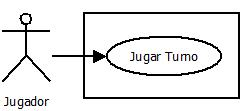
\includegraphics[width=8cm, height=4cm]{imgs/DiagramaCasoUso1.png}}
	\subfloat[Diagrama N°2]
	{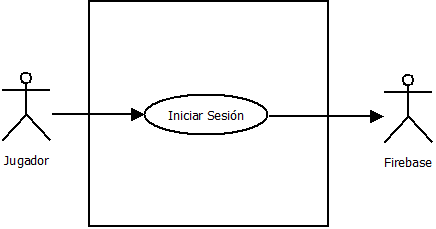
\includegraphics[width=8cm, height=4cm]{imgs/DiagramaCasoUso2.png}}
 	\caption{Digramas de casos de uso 1 y 2}
\end{figure}

\begin{figure}[H]
	\centering
	Los siguientes diagramas hacen referencia a los casos de uso 3 y 4 respectivamente\\(Tablas \ref{Caso_de_uso_3} y \ref{Caso_de_uso_4})
	\subfloat[Diagrama N°3]
	{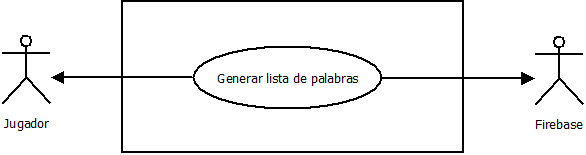
\includegraphics[width=8cm, height=4cm]{imgs/DiagramaCasoUso3.png}}
	\subfloat[Diagrama N°4]
	{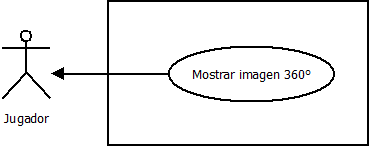
\includegraphics[width=8cm, height=4cm]{imgs/DiagramaCasoUso4.png}}
 	\caption{Digramas de casos de uso 3 y 4}
\end{figure}

\begin{figure}[H]
	\centering
	Los siguientes diagramas hacen referencia a los casos de uso 5 y 6 respectivamente\\(Tablas \ref{Caso_de_uso_5} y \ref{Caso_de_uso_6})
	\subfloat[Diagrama N°5]
	{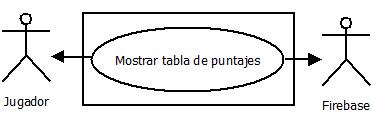
\includegraphics[width=8cm, height=4cm]{imgs/DiagramaCasoUso5.png}}
	\subfloat[Diagrama N°6]
	{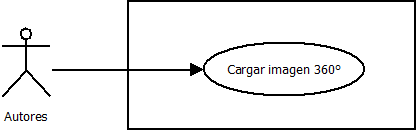
\includegraphics[width=8cm, height=4cm]{imgs/DiagramaCasoUso6.png}}
 	\caption{Digramas de casos de uso 5 y 6}
\end{figure}

\begin{figure}[H]
\centering
	Este diagrama muestra como serian todos los diagramas vistos anteriormente en un formato generalizado y en convivencia con todos los demás y como interactúan entre si.\\
	\bigskip\bigskip
   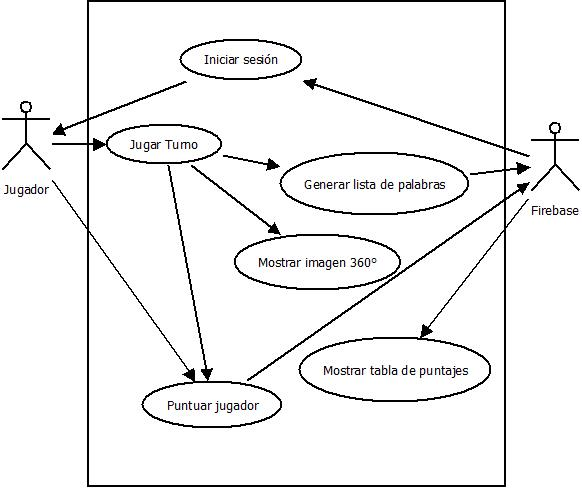
\includegraphics[scale=0.7]{imgs/DCUs.jpeg}
   \begin{center}
   \caption{Diagrama general de casos de uso}
   \end{center}
\end{figure}

\subsubsection{Contrato}
Los contratos describen que es lo que se espera de una operación, enfatizando más en el análisis que en el diseño, es decir, responde principalmente al "¿Que debe hacer el sistema?". Para esto, es común utilizar pre y postcondiciones que giran en torno a los cambios de estado.
Estos contratos son, en resumidas cuentas, una forma de presentar funciones o acciones concretas y un tanto especificas de lo que hace nuestro software.

A continuación presentamos algunos de ellos.

\begin{table}[H]
    \begin{center}
        \begin{tabular}{| m{15cm} |}       
        	\hline 
        	\textbf{Nombre:} Inicio del juego \\
        	\hline
        	\textbf{Responsabilidades:} Comunicarle al usuario de que la aplicación se a iniciado\\
        	\hline
        	\textbf{Tipo:} Pantalla inicial \\
        	\hline
        	\textbf{Referencias cruzadas:} Nulo\\
        	\hline
        	\textbf{Caso de uso:} Nulo\\
        	\hline
        	\textbf{Notas:} \\
        	\hline
        	\textbf{Excepciones:} \\
        	\hline
        	\textbf{Salida:} \\
        	\hline
        	\textbf{Precondiciones:} La aplicación se inicia con ningún tipo de error\\
        	\hline
        	\textbf{Poscondiciones:} Se entrega acceso a el uso de la aplicación luego de verificar y autentificar los datos. Referencia a tabla \ref{Caso_de_uso_2}\\
        	\hline
        \end{tabular}
	\caption{Contrato: inicio de juego}
    \label{Contrato1}
    \end{center}
\end{table}

\begin{table}[H]
    \begin{center}
        \begin{tabular}{|m{15cm} |}         
        	\hline 
        	\textbf{Nombre:} Inicio de sesion \\
        	\hline
        	\textbf{Responsabilidades:} Reconocer al usuario o entregarle la posibilidad de crear un perfil para ingresar al juego\\
        	\hline
        	\textbf{Tipo:} Sistema \\
        	\hline
        	\textbf{Referencias cruzadas:} R1.1 R1.2\\
        	\hline
        	\textbf{Caso de uso:} 2. Iniciar sesión\\
        	\hline
        	\textbf{Notas:} Existe un mensaje de error al ingresar datos incorrectos\\
        	\hline
        	\textbf{Excepciones:} Nulo\\
        	\hline
        	\textbf{Salida:} Se avisa a la base de datos el ingreso de un usuario al sistema\\
        	\hline
        	\textbf{Precondiciones:} La aplicación debe tener una conexion con la base de datos para reconocer al usuario \\
        	\hline
        	\textbf{Poscondiciones:} Se obtuvo los datos del usuario y se avisa de su ingreso a la aplicación\\
        	\hline
        \end{tabular}
    \caption{Contrato: inicio de sesión}
    \label{Contrato2}
    \end{center}
\end{table}

\begin{table}[H]
    \begin{center}
        \begin{tabular}{| m{15cm} |}            
        	\hline 
        	\textbf{Nombre:} Lista de palabras \\
        	\hline
        	\textbf{Responsabilidades:} Generar una lista de palabras al azar y entregarselas a los usuarios\\
        	\hline
        	\textbf{Tipo:} Sistema\\
        	\hline
        	\textbf{Referencias cruzadas:} R1.5 R1.8\\
        	\hline
        	\textbf{Caso de uso:} 3. Generar lista de palabras\\
        	\hline
        	\textbf{Notas:} \\
        	\hline
        	\textbf{Excepciones:} Nulo \\
        	\hline
        	\textbf{Salida:} Nulo\\
        	\hline
        	\textbf{Precondiciones:} La aplicación contiene una cantidad minima de palabras a elegir y una conexión con los usuarios\\
        	\hline
        	\textbf{Poscondiciones:} Se generan las palabras y se entregan a los usuarios\\
        	\hline
        \end{tabular}
    \caption{Contrato: Lista de palabras}
    \label{Contrato3}
    \end{center}
\end{table}

\begin{table}[H]
    \begin{center}
        \begin{tabular}{| m{15cm} |}       
        	\hline 
        	\textbf{Nombre:} Pantalla imagen 360°\\
        	\hline
        	\textbf{Responsabilidades:} Se ve la imagen en 360 en cada partida \\
        	\hline
        	\textbf{Tipo:} Visual\\
        	\hline
        	\textbf{Referencias cruzadas:} R1.3\\
        	\hline
        	\textbf{Caso de uso:} 4. Mostrar imagen 360°\\
        	\hline
        	\textbf{Notas:} Se debe mover el dispositivo físico para apreciar la imagen completa\\
        	\hline
        	\textbf{Excepciones:} Nulo \\
        	\hline
        	\textbf{Salida:} Nulo \\
        	\hline
        	\textbf{Precondiciones:} Debe existir una imagen cargada previamente y los usuarios que verán esta \\
        	\hline
        	\textbf{Poscondiciones:} Se entrefa la imagen con la opción de finalizar su visualización\\
        	\hline
        \end{tabular}
    \caption{Contrato: Pantalla imagen 360°}
    \label{Contrato4}
    \end{center}
\end{table}

\begin{table}[H]
    \begin{center}
        \begin{tabular}{| m{15cm} |}        
        	\hline 
        	\textbf{Nombre:} Presentación de puntajes \\
        	\hline
        	\textbf{Responsabilidades: }Entregar feedback luego de la realización de un turno \\
        	\hline
        	\textbf{Tipo:} Sistema \\
        	\hline
        	\textbf{Referencias cruzadas:}R1.8 \\
        	\hline
        	\textbf{Caso de uso:} 5. Mostrar tabla de puntajes\\
        	\hline
        	\textbf{Notas:} \\
        	\hline
        	\textbf{Excepciones:} Nulo \\
        	\hline
        	\textbf{Salida:} Puntaje en base a la valoración de los usuarios\\
        	\hline
        	\textbf{Precondiciones:}  accede a la tabla de puntajes y el programa a su vez se ingresae este valor a la base de datos \\
        	\hline
        	\textbf{Poscondiciones:} Los puntajes se analizan y se entregan a los usuarios\\
        	\hline
        \end{tabular}
    \caption{Contrato: Presentación de puntajes}
    \label{Contrato5}
    \end{center}
\end{table}

\begin{table}[H]
    \begin{center}
        \begin{tabular}{| m{15cm} |}          
        	\hline 
        	\textbf{Nombre:} Cargar imagen 360°\\
        	\hline
        	\textbf{Responsabilidades:} Carga de una imagen en 360 para ser visualizada por los usuarios\\
        	\hline
        	\textbf{Tipo:} Sistema\\
        	\hline
        	\textbf{Referencias cruzadas:} R1.7\\
        	\hline
        	\textbf{Caso de uso:} 6. Cargar imagen 360°\\
        	\hline
        	\textbf{Notas:} Nulo\\
        	\hline
        	\textbf{Excepciones:} La ruta de la imagen debe exisitir de lo contrario no funciona\\
        	\hline
        	\textbf{Salida:} Nulo\\
        	\hline
        	\textbf{Precondiciones:} Una imagen de 360 \\
        	\hline
        	\textbf{Poscondiciones:} La imagen esta lista para ser presentada al momento de que los usuarios ingresen\\
        	\hline
        \end{tabular}
    \caption{Contrato: Cargar imagen 360°}
    \label{Contrato6}
    \end{center}
\end{table}

\subsubsection{Modelo Conceptual}
El modelo conceptual que se presenta a continuacion muestra las relaciones que hay entre los diversos organismos, clases y conceptos dentro del software. Presenta como es el flujo entre cada uno de los miembros, es decir, que relacion tiene cada uno de los conceptos. La forma escrita de representarlo seria:
El mapa de juego(lo que vendria siendo el tablero), contiene imagenes 360° y a su ves requiere poder usar el fire base para poder usar la base de datos, quien a su vez almacena palabras, jugadores y una tabla de puntajes.
\begin{figure}[H]
\centering
   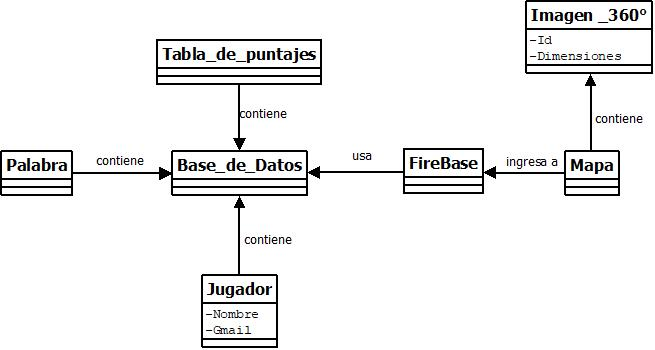
\includegraphics[scale=0.9]{imgs/ModeloConceptual.jpeg}
   \caption{Modelo conceptual}
\end{figure}
\newpage
\subsubsection{Diagrama de Secuencia o Colaboración}
Los función y proposito de los siguientes diagramas de secuencia o colaboración sirven para ejemplificar de manera grafica y como apoyo visual la comunicación entre los autores y el sistema de cada caso de uso.
\begin{figure}[H]
	\centering
	Los siguientes diagramas hacen referencia a los casos de uso 1 y 2 respectivamente\\(Tablas \ref{Caso_de_uso_1} y \ref{Caso_de_uso_2})
	\subfloat[Diagrama de secuencia N°1]
	{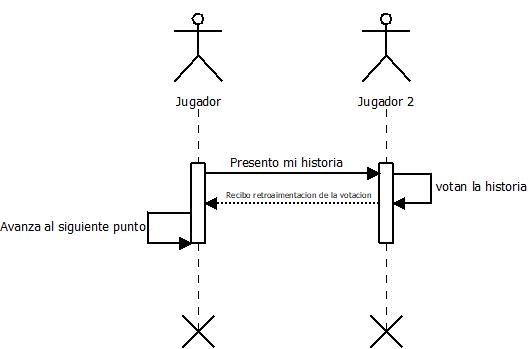
\includegraphics[width=8cm, height=6cm]{imgs/DS_1.jpeg}}
	\subfloat[Diagrama de secuencia N°2]
	{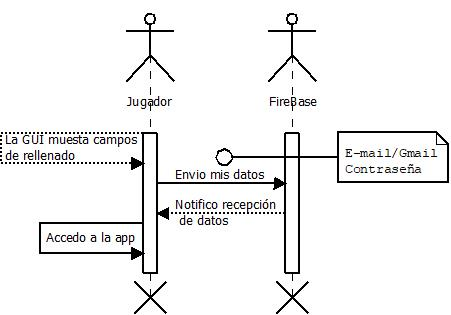
\includegraphics[width=8cm, height=6cm]{imgs/DS_2.jpeg}}
 	\caption{Digramas de secuencia 1 y 2}
\end{figure}

\begin{figure}[H]
	\centering
	Los siguientes diagramas hacen referencia a los casos de uso 3 y 4 respectivamente\\(Tablas \ref{Caso_de_uso_3} y \ref{Caso_de_uso_4})
	\subfloat[Diagrama de secuencia N°3]
	{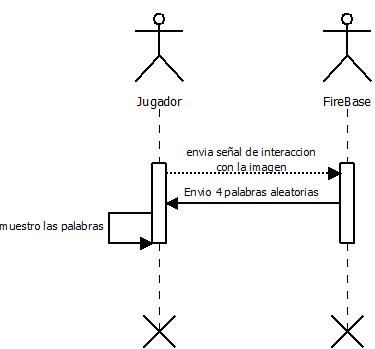
\includegraphics[width=8cm, height=6cm]{imgs/DS_3.jpeg}}
	\subfloat[Diagrama de secuencia N°4]
	{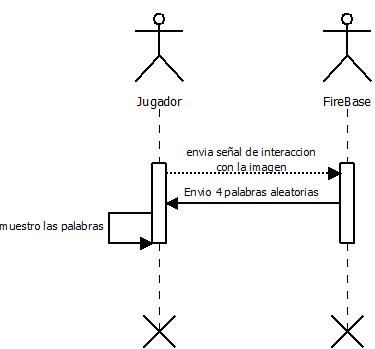
\includegraphics[width=8cm, height=6cm]{imgs/DS_3.jpeg}}
 	\caption{Digramas de secuencia 3 y 4}
\end{figure}

\begin{figure}[H]
	\centering
	Los siguientes diagramas hacen referencia a los casos de uso 5 y 6 respectivamente\\(Tablas \ref{Caso_de_uso_5} y \ref{Caso_de_uso_6})
	\subfloat[Diagrama de secuencia N°5]
	{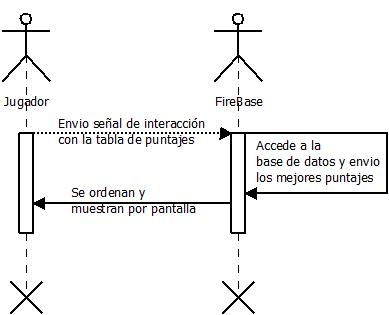
\includegraphics[width=8cm, height=6cm]{imgs/DS_5.jpeg}}
	\subfloat[Diagrama de secuencia N°6]
	{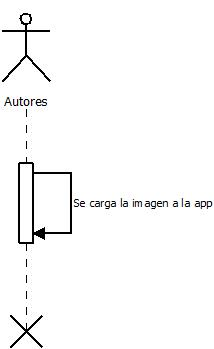
\includegraphics[width=8cm, height=6cm]{imgs/DS_6.jpeg}}
 	\caption{Digramas de secuencia 5 y 6}
\end{figure}

\subsubsection{Priorización}
Para tener claridad de los que nos resulta mas apremiante o necesario para el software necesitamos tener muy presente el motivo de su creación, que queremos lograr con su desarrollo. Es por esto que debemos evaluar las funciones de nuestro juego y hacernos la gran pregunta "Si elimino esto, ¿Seguira funcionando la aplicación", si la respuesta es \textbf{NO}, entonces nos encontramos con una parte \textbf{Escencial} para nuestro software, ahora, en caso de que la respuesta sea si,  "¿Sigue siendo jugable? o ¿Entiendo como proseguir si lo borro?", en caso de que la respuesta sea una negativa entonces tambien cuenta como un atributo \textbf{Escencial} para el desarrollo.
Ahora bien, todos los elementos esteticos cuya función es simplemente la de hacer mas agradable y comprensible todo el resto de funciones, forman parte de atributos o funciones \textbf{Importantes}.

Los siguientes son los proncipales funciones y caracteristicas con las que nuestro software debe contar, utilizando el metodo de priorizacion antes mencionado.

\begin{enumerate}[1.]
	\item Jugar una partida de Conquista Turística 360° \textbf{Esencial}.
	\item Iniciar sesión \textbf{Esencial}
	\item Generar lista de palabras \textbf{Esencial}
	\item Mostrar imagen 360 \textbf{Esencial}
	\item Mostrar tabla de puntajes \textbf{Importante}
	\item Cargar imagen 360° \textbf{Esencial}
\end{enumerate}

\subsection{Modelo de Dominio}
El modelo de dominio presentado cumple con la presentacion de manera conceptual de todas las clases dentro de nuestro sistema, con el fin de que se comprenda la relacion ente los objetos del mundo real que se tienen y como estos afectan a nuestro desarrolllo y visión de programa, o, en otras palabras, como tomamos importancia de hacer que nuestra software sea lógico y cumpla a su vez con un modelo de programación facil de comprender, aproximandose lo mas posible a lo que significa programación orientada a objetos.
\subsubsection{Entidades Reconocidas}
Dentro de este software solo pudimos identificar a la base de datos como una entidad, tomando en consideración lo que entendemos por entidad.
Base de Datos: Sistema de almacenamiento de recursos necesarios para el funcionamiento de la aplicación.
\subsubsection{Modelo de Dominio}
\begin{figure}[H]
\centering
   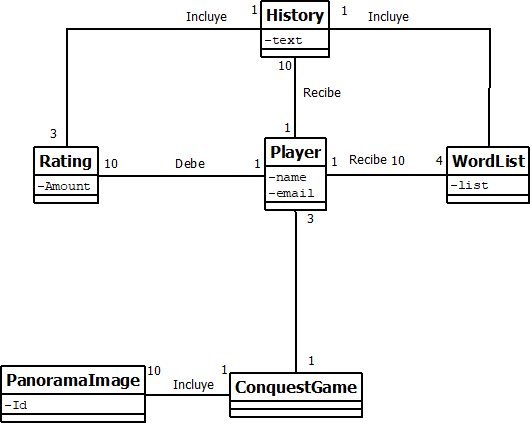
\includegraphics[width=14cm, height=6cm]{imgs/ModeloDominio.png}
   \begin{center}
   \caption{Diagrama de dominio: UML}
   \end{center}
\end{figure}
\subsubsection{Matriz de Rastreabilidad}

\begin{table}[H]
    \centering
	\begin{tabular}{| c | c | c | c | c | c | c |}       
		\hline 
		& History & Rating & Player & WordList & PanoramaImage & ConquestGame\\
		\hline
		1 & X & X & X & X & X & X \\
		\hline
		2 &  & & X &  &  &  \\
		\hline
		3 &  &  &  & X &  &  \\
		\hline
		4 &  &  &  &  & X &  \\
		\hline
		5 &  & X &  &  &  &  \\
		\hline
		6 &  &  &  &  & X &  \\
		\hline
	\end{tabular}
	\caption{Matriz de rastreabilidad}
\end{table}